\documentclass{scrartcl}
\usepackage{scrlayer-scrpage}
\usepackage[czech]{babel}
\usepackage{amsmath}
\usepackage{graphicx}

\cohead[ADS 2]{ADS 2}
\lohead[Všemocný NAND]
        {Všemocný NAND}
\rohead[Václav Luňák (Vašek)]
        {Václav Luňák (Vašek)}
\pagestyle{plain.scrheadings}

\graphicspath{ {./ukol8_imgs/} }

\begin{document}

\textit{V následující úloze jsou NAND hradla značena čísly a vstupy malými písmeny.}
\section{XOR}
Hradlo XOR reprezentujeme následující sítí:

\begin{center}
    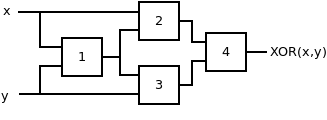
\includegraphics[width=0.5\linewidth]{nand_to_xor}
\end{center}

Důkaz správnosti obvodu provedeme rozborem všech možných vstupů.

\begin{center}
    \begin{tabular}{ c | c | c | c | c | c | c }
        x & y & 1 & 2 & 3 & 4 & XOR \\ \hline
        0 & 0 & 1 & 1 & 1 & 0 & 0   \\
        0 & 1 & 1 & 1 & 0 & 1 & 1   \\
        1 & 0 & 1 & 0 & 1 & 1 & 1   \\
        1 & 1 & 0 & 1 & 1 & 0 & 0   
    \end{tabular}
\end{center}

\section{Booleovské obvody}
Víme, že každý booleovský obvod se dá sestavit pomocí hradel $NOT$, $AND$ a $OR$. Stačí nám tedy pomocí $NAND$ reprezentovat tato tři hradla. To provedeme následovně:

\begin{figure}[!htb]
    \minipage{0.3\textwidth}
      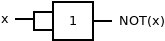
\includegraphics[width=\linewidth]{nand_to_not}
    \endminipage\hfill
    \minipage{0.3\textwidth}
      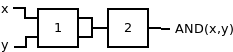
\includegraphics[width=\linewidth]{nand_to_and}
    \endminipage\hfill
    \minipage{0.3\textwidth}
      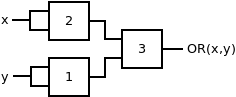
\includegraphics[width=\linewidth]{nand_to_or}
    \endminipage
\end{figure}

Zbývá dokázat ekvivalenci těchto sítí s jejich příslušnými hradly.

\begin{center}
    \begin{tabular}{c | c | c}
        x & 1 & NOT \\ \hline
        0 & 1 & 1   \\
        1 & 0 & 0         
    \end{tabular}
    \hspace{10pt}
    \begin{tabular}{c | c | c | c | c}
        x & y & 1 & 2 & AND \\ \hline
        0 & 0 & 1 & 0 & 0   \\
        0 & 1 & 1 & 0 & 0   \\
        1 & 0 & 1 & 0 & 0   \\
        1 & 1 & 0 & 1 & 1   
    \end{tabular}
    \hspace{10pt}
    \begin{tabular}{c | c | c | c | c | c}
        x & y & 1 & 2 & 3 & OR  \\ \hline
        0 & 0 & 1 & 1 & 0 & 0   \\
        0 & 1 & 0 & 1 & 1 & 1   \\
        1 & 0 & 1 & 0 & 1 & 1   \\
        1 & 1 & 0 & 0 & 1 & 1
    \end{tabular}
\end{center}

\end{document}
